\section{Results and Discussion}\label{sec:results}

\begin{figure*}[!b]
\centering
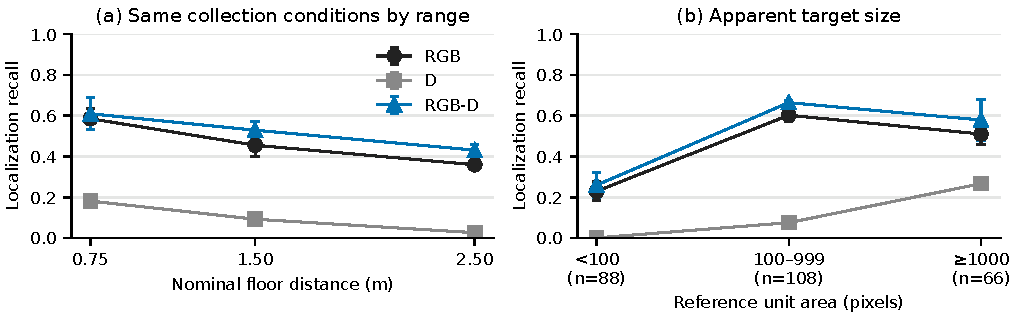
\includegraphics[width=\textwidth]{figures/range_and_size.pdf}
\caption{ESANet reference-supervised localization by (a) nominal floor distance and (b) reference-mask area. Points show three-seed means; bars show seed standard deviation, not independent-scene confidence intervals. Panel (a) averages the five static repeats within each of 20 recordings per distance. Panel (b) averages repeats within reference-unit/recording pairs; $n$ includes explicit object groups. Pixel size, category and distance covary. All predictions use full images; recording props remain in the diagnostic domain.}
\label{fig:range-size}
\end{figure*}

\subsection{Experimental comparisons}

We evaluate the completed runs on all 320 GTE-Floor frames, without
fine-tuning on these recordings. Table~\ref{tab:results} reports the
reference-supervised comparators and the accepted three-prompt SAM
supervision. ESANet uses three seeds per condition, except automatic
RGB, for which two completed seeds are available. Supervision changes
are compared using matching seeds only. Historical SAM-label versions
are excluded from this comparison. The RGB-D repeats use the same
PyTorch 2.10 version as the RGB and D experiments.

\begin{table}[H]
\caption{GTE-Floor diagnostic results. IoU and recalls are percentages. IoU and localization recall $R_{\mathrm{loc}}$ (adjusted IoU $\geq0.5$) show mean $\pm$ seed standard deviation. Coverage recall $R_{\mathrm{cov}}$ (at least half the target covered) and false components/frame (FC) show means. $n$ counts seeds; direct methods are fixed. Full frames include props, with no area filter. SAM uses the three-prompt labels.}
\label{tab:results}
\centering
\footnotesize
\setlength{\tabcolsep}{2.5pt}
\begin{tabular}{@{}lrcccc@{}}
\toprule
Model / labels & $n$ & IoU & $R_{\mathrm{cov}}$ & $R_{\mathrm{loc}}$ & FC \\
\midrule
RGB / reference & 3 & 48.6 $\pm$ 7.5 & 62.8 & 45.4 $\pm$ 1.8 & 3.65 \\
D / reference & 3 & 14.1 $\pm$ 1.2 & 38.3 & 9.8 $\pm$ 1.2 & 8.24 \\
RGB-D / reference & 3 & 55.4 $\pm$ 8.8 & 64.3 & 50.7 $\pm$ 4.6 & 2.84 \\
RGB / SAM & 2 & 46.8 $\pm$ 3.0 & 75.2 & 60.1 $\pm$ 0.2 & 5.76 \\
D / SAM & 3 & 12.6 $\pm$ 1.8 & 36.3 & 9.7 $\pm$ 2.0 & 8.82 \\
RGB-D / SAM & 3 & 49.8 $\pm$ 3.7 & 75.3 & 60.7 $\pm$ 1.6 & 6.03 \\
U-Net / reference & 3 & 48.5 $\pm$ 1.5 & 52.0 & 44.4 $\pm$ 1.5 & 3.18 \\
YOLO / reference & 3 & 45.9 $\pm$ 1.0 & 60.0 & 47.1 $\pm$ 3.3 & 1.01 \\
Direct SAM & -- & 41.8 & 94.5 & 84.0 & 2.54 \\
Floor fit & -- & 3.8 & 69.5 & 5.7 & 344.02 \\
\bottomrule
\end{tabular}
\end{table}

\subsection{Contribution of depth and object scale}

Reference-supervised RGB-D reaches mean GTE-Floor IoU 0.554, compared
with 0.486 for RGB and 0.141 for D. The paired RGB-D minus RGB IoU
changes range from $-6.3$ to $+20.3$ percentage points across seeds;
the mean gain of 6.8 points is therefore not consistent across runs.
Localization recall increases from 0.454 to 0.507, while coverage recall
changes only from 0.629 to 0.643: tighter localization is not necessarily
a newly recovered object. The mean localization advantage persists at
overlap thresholds 0.25, 0.50 and 0.75 (4.2, 5.3 and 5.8 points).
U-Net and YOLO provide comparable RGB results, with different
localization/false-component tradeoffs (Table~\ref{tab:results}).
On the limited 30-frame reviewed ISOD test subset, RGB and RGB-D mean
IoU are 0.754 and 0.753; these provisional scores do not establish a
fusion advantage on the full test split.

In Fig.~\ref{fig:range-size}(a), mean recording-level localization
recall falls from 0.585 to 0.359 for RGB between the 0.75 and 2.5 m
marks, from 0.610 to 0.431 for RGB-D, and from 0.181 to 0.026 for D.
Small apparent targets are also difficult to localize (Fig.~\ref{fig:range-size}(b)).
The observations support a range/scale limitation, but distance changes
pixel area and viewpoint together; they do not isolate depth noise.

\begin{figure*}[!t]
\centering
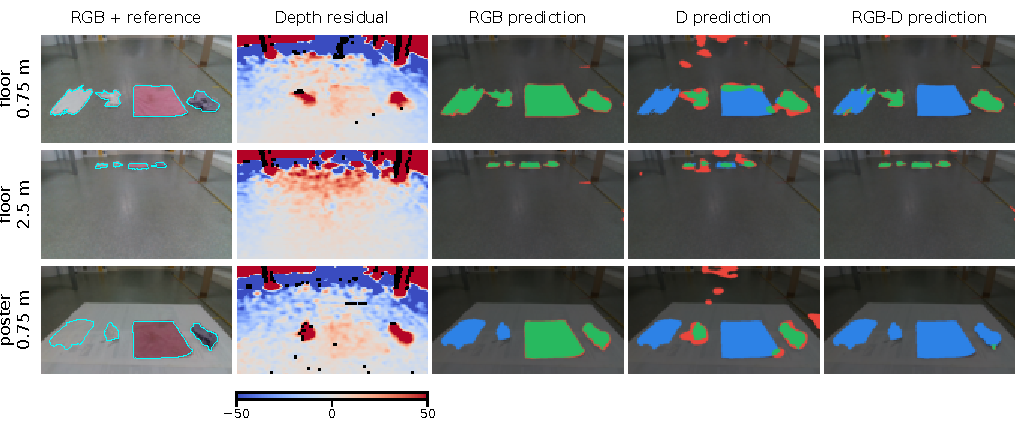
\includegraphics[width=\textwidth]{figures/cloth_depth_examples.pdf}
\caption{Matched cloth/tissue views: near/far bare floor and the near white poster, using the 52 cm camera configuration, frame 2 and seed 0. All rows retain the same full-image scale. Cyan outlines show the reference; prediction colors are green for correct foreground, blue for missed foreground and red for extra foreground. Residuals share a $[-50,50]$ mm scale; black marks unavailable values. This camera-axis floor-fit residual is not physical height. The leftmost flat towel has little positive near residual, unlike the adjacent crumpled tissue. Fusion misses flat foreground in the near floor view despite RGB success; neither model rescues the flat white towel on the poster.}
\label{fig:cloth-depth}
\end{figure*}

\subsection{Qualitative evidence and depth reliance}

Figure~\ref{fig:cloth-depth} illustrates why valid depth is not the
same as a useful obstacle cue. At the near mark, median valid-depth
fractions exceed 0.99 for both the flat paper towel and crumpled tissue,
but their median object-versus-nearby-floor residual differences are
approximately $-0.8$ and $+43.5$ mm. Across all seeds and repeats, D
localizes the near crumpled tissue but misses the flat towel at all
three marks. RGB localizes both throughout; RGB-D misses the near towel
in one seed. This is descriptive, not a controlled folding experiment:
the items differ in material, shape and area.

In matched floor/poster recordings, the flat white towel is missed on
the poster by both RGB and RGB-D across all seeds and repeats, despite
frequent localization on bare floor. Its nearby-floor color difference
also decreases. This is a difficult low-contrast case, not evidence that
depth compensates for missing RGB contrast; background context changes
alongside appearance.

Keeping RGB and model weights fixed, replacing depth with missing
readings reduces mean RGB-D IoU from 0.554 to 0.147. However, permuting
depth between object sets within the same camera/background/distance
configuration gives 0.547. Missing depth is an out-of-distribution
input, while the permutation preserves much scene geometry. Thus the
zero-depth degradation alone does not demonstrate use of precise
object-level depth; these checks measure reliance under interventions.

\subsection{Automatic supervision and limitations}

For RGB-D, replacing reference training masks with the RGB-only SAM
labels changes mean IoU from 0.554 to 0.498, but raises localization
recall from 0.507 to 0.607, coverage recall from 0.643 to 0.753, and
false components from 2.84 to 6.03 per frame. The gain in recovered reference units is accompanied by more
excess detections, rather than an unqualified improvement. RGB shows
the same recall/false-component tradeoff on its two matched seeds;
D remains weak with either supervision. Direct SAM localizes 0.840 of
reference units but reaches only 0.418 pixel IoU. Detection and boundary
accuracy therefore require separate reporting.

Teacher-mask pooled IoU is 0.604 on 300 reviewed validation frames and
0.757 on 30 reviewed test frames. Validation informed prompt selection,
so its quality estimate is not independent. A retrospective 370-frame
reference-assistance replay gives mean image IoU 0.878; a later 14-frame
random check gives 0.837 with two major errors. Both reference assistance
and the teacher use SAM, so correlated annotation errors can remain
after review. GTE-Floor covers one room; camera height and tilt change
together. Grouped references and recording props limit the full-frame
diagnostic; it is not operational accuracy or instance AP.

\section{Conclusion and Future Work}\label{sec:conclusion}

RGB appearance provides a strong floor-obstacle baseline. RGB-D improves
average external localization and IoU, but its gain varies across seeds
and is not supported by every object example. Depth alone struggles
with small, flat and distant targets. Automatic SAM labels can train
models that recover more reference units, with a substantial
false-component cost. Future work should expand reviewed ISOD test
coverage, verify instance/group annotations, and evaluate fixed
collection-area crops with recording props handled explicitly. Those
steps are needed before claiming reliable individual-object detection
or deployment performance.
